%% TestVDB — FSE 2027 submission, measurement/experience register (2026-09-15).
%% Source of truth for the prose: docs/paper-sample-lqm-path.md (sample v10).
%% Every number here is reproduced by scripts shipped in the replication package:
%%   rq2/analyses/{recompute_paper_numbers,clause_tally,convention_pricing,
%%                 bootstrap_net_f1}.py and rq2/analyses/audit/pair_audit.py
%% FSE 2027 format: acmsmall single-column, 18 pages text+figures + 4 pages refs.
%% Deadline: 2026-10-02 AoE. Data Availability section required after Conclusion.
\documentclass[acmsmall,screen,review,anonymous]{acmart}

\usepackage{tikz}
\usetikzlibrary{positioning, arrows.meta}
\emergencystretch=2em
\settopmatter{printacmref=false}
\settopmatter{printfolios=false}
\newcommand{\system}{TestVDB}

\begin{document}

\title[TestVDB: Mining Documentation--Implementation Bugs in Vector Databases]{TestVDB:
Using LLMs to Mine Documentation--Implementation Bugs in Vector Database Management Systems}

\begin{abstract}
Vector Database Management Systems (VDBMSs) fail mostly without crashing, and the one dedicated
VDBMS fuzzer is crash-oracle by construction, so the silent documentation--implementation bugs they
admit are out of its reach by design. We report a mining campaign, an audit of the evidence its
confirmation stage reads, and a census of that stage's errors.

\textbf{The campaign.} Across Milvus, Qdrant, and Weaviate, maintainers confirmed \textbf{51 of 81}
adjudicated submissions and fixed 23 through merged PRs, over 16 of the ledger's 19 versions. It is a
record of submissions and adjudication, \emph{not} a per-run detection rate: the runs that would have
measured detection ability were voided for dispatch-discipline violations, and nothing here depends on
them.

\textbf{The audit.} The packages that stage reads are distilled from vendor documentation. Auditing
their 134 (constraint, cited-page) pairs---as the pipeline produced them, before the repair---against
the page each cites: \textbf{18 are supported as cited, 58 cite a source file or a landing page and
were re-anchored, and 58 have no support on their cited page}---43.3\%. The same audit exposed two
leak channels, since repaired and the affected cases re-judged; \textbf{every rate below is computed
on the cleaned pool}.

\textbf{The census.} Classifying the deployed stage's 243 judgments by the clause that closes them
locates the error budget in the one refuting clause its protocol does not guard---measured on the
primary backbone, and not reproduced on the second. Contract refutation carries no evidence
requirement, closes 50 judgments, and 24 of them are maintainer-confirmed bugs; verbatim-guarded
by-design refutation closes 19 and is right 17 times. \textbf{80\% of the stage's incorrect closures
to False-Positive come from the unguarded clause}; routing it instead of closing on it recovers seven
true bugs for nine more false positives released.
\end{abstract}

\maketitle

\section{Introduction}
\label{sec:intro}

VDBMSs such as Milvus, Qdrant, and Weaviate store the embeddings that retrieval-augmented LLM
applications depend on. When a VDBMS query is buggy the wrong context reaches the model---a disabled
filter returns all matches, a zero-length vector corrupts an index---and the error propagates with
no crash and no error code to log. Empirical studies agree this is the dominant shape: most VDBMS
bugs are functional failures that keep the service up while returning wrong results, and the one
dedicated VDBMS fuzzer is crash-oracle by construction.

We target a prevalent subset: \emph{documentation--implementation bugs}, where a VDBMS silently
accepts an input or produces a behavior that violates its API documentation. A canonical instance:
Milvus documents \texttt{nprobe} as an integer in $[1, 16384]$, yet the search API accepts
\texttt{nprobe=0} with HTTP 200 and returns results (issue \#49823).

Detecting such bugs requires an expectation derived from the documentation prose, and no
deterministic-oracle family we analyze anchors its expectation there. Reading prose is a
semantic-interpretation step only an LLM currently performs at scale---which imports the LLM's
false-positive problem, because the same model family that misreads an ambiguous sentence into an
over-strong constraint later judges whether the observed behavior violates it. \textbf{Both halves
of that sentence are measurable, and we measure both}: what the distillation keeps from the
documentation, and where the confirmation stage makes its errors.

We contribute:

\begin{enumerate}
  \item \textbf{A mining campaign with maintainer-validated yield} across three production VDBMSs:
    maintainers confirmed 51 of 81 adjudicated submissions (Milvus 29, Qdrant 14, Weaviate 8) and
    fixed 23 through merged PRs, over 16 of the ledger's 19 versions. It carries our own screening
    and submission decisions, and the runs that would have measured per-version detection ability
    were voided for dispatch-discipline violations; nothing here depends on them.
  \item \textbf{An audit-and-rebuild discipline for documentation-derived oracle material}, with the
    first quantitative pair-level measurement we know of for how much of it is unsupported by its own
    citations. Of the 134 (constraint, cited-page) pairs the packages carry as the pipeline produced
    them, \textbf{18 are supported as cited, 58 cite a source file or an API landing page and were
    re-anchored, and 58 have no support on their cited page}; on the 12 case-level main assertions, a
    separate object, the audit acted on all 12. Two leak repairs followed from it, and every rate
    below is computed on the cleaned pool.
  \item \textbf{A clause-level error census} of the confirmation stage, locating the evidence guard
    on the wrong clause: contract refutation carries no evidence requirement, closes 50 of the
    stage's 243 judgments, and \textbf{24 of them are real bugs}---\textbf{80\% of the stage's
    incorrect closures to False-Positive}---while the verbatim-guarded by-design clause closes 19 and
    is right 17 times. Routing the unguarded clause instead of closing on it recovers seven true bugs
    and releases nine more false positives under the deployment's convention. The census is measured
    on the primary backbone and does not reproduce on the second; Section~\ref{sec:census} states
    that scope and identifies the two refuting clauses by the evidence their cells carry.
\end{enumerate}

We also report defects in our own instrument. Four defects in our own dispatches were found by
reviewers reading the shipped texts, not by us: eight of twelve declare an output field that
contradicts their own verdict vocabulary; the deployed dispatch prints two aggregation rules with
opposite defaults and defines the four perspectives twice with C and D exchanged; and its output
schema declares the source vocabulary for a perspective the text calls maintainer cognition, which
98 of 243 recorded cells use. We report them because the paper's methodological claim is that this
pipeline is auditable, and an audit that only reports what it finds in the target is not one.

\section{Preliminaries}
\label{sec:prelim}

\textbf{The non-crashing majority.} Studies of VDBMS defects converge on one structural fact: most
do not crash. The systematic bug study attributes the dominant share to functional failures---the
service stays up and silently returns wrong results---with crash-producing defects a minority class
\cite{bugstudy25,roadmap25}. The one dedicated VDBMS fuzzer, VDBFuzz, reaches exactly that minority:
its oracle fires on a 5xx response or a failed request induced by template-driven input mutation,
not on the silent misbehaviour at issue here \cite{vdbfuzz26}. The community roadmap names oracle
definition as the open problem for what is left \cite{roadmap25}, and that residual is where this
paper works.

\textbf{What we target.} The subset we study is \emph{documentation--implementation inconsistency}:
the system silently accepts an input, errors where it documented success, returns a shape its API
reference does not describe, or leaves state the documentation says cannot arise. We separate this
from \emph{correctness}. Consistency asks whether observable behavior matches what the documentation
prescribes---what is accepted, rejected, returned, how state evolves; correctness asks whether a
result is right in the mathematical sense, such as whether an approximate search returns the true
top-$k$. Vector-search correctness is not what this paper measures, and the two are checked by
different means.

The reverse shape also occurs and is harder to see: an operation documented as all-or-nothing applies
partially, or a transition---delete, recreate, restore---leaves behavior the documentation does not
allow. These are the silent majority's own subclass, and none produces a signal a crash oracle can
fire on.

\textbf{Why the expectation has to be read from prose.} Every testing oracle needs an expectation,
and oracle families differ in where they get one. Table~\ref{tab:oracles} lists the candidates
relevant here and the structural reason each anchors somewhere other than system-level API prose.

\begin{table}[t]
\caption{Oracle candidates, where each anchors its expectation, and why it misses the
documentation--implementation residual.}
\label{tab:oracles}
\footnotesize
\begin{tabular}{@{}p{0.20\textwidth}p{0.24\textwidth}p{0.46\textwidth}@{}}
\toprule
Candidate oracle & Expectation anchored in & Why it misses this residual \\
\midrule
crash signal (VDBFuzz) & process death or 5xx & the bugs here do not crash \\
differential testing (NoREC, TLP, DQE) & another evaluation of the same engine, or another vendor &
intra-system variants compare an engine with itself and derive nothing from documentation;
cross-vendor behavior diverges by design \\
metamorphic relations & a relation the tester already poses & deriving \emph{which} relation the
prose prescribes is the semantic step non-LLM tooling does not perform \\
property-based testing, schemas & field types, declared ranges, enum sets & a schema bounds fields;
it does not carry cross-request or state-coupling behaviour, and where a schema declares a minimum it
may omit the maximum that matters \\
structured-source oracles (AGORA+, SATORI, MASTOR, MASTEST) & OpenAPI fields, execution traces, or
the implementation source & anchored in structured sources, at or below field granularity; the
source-anchored members encode implemented behaviour, and none takes untagged, system-level
behavioural prose as its statement of intent \\
documentation-derived oracles (@tComment, JDoctor, DocTer, RBCTest, RESTInfer) & tagged or
method-/parameter-level prose & prose-derived, but the derived oracle stays the final arbiter and
the granularity sits below system-level behavioural prose \\
\bottomrule
\end{tabular}
\end{table}

Each of these reaches something real. The point of the table is narrower: the families that read
prose at all read it at field, parameter or method granularity, and often from tagged sources; none
of them takes its expectation from \textbf{untagged, system-level behavioural prose}, which is where
the VDBMS documentation states the constraints that matter here---``the other collection should have
the same vector size as the current one'', an \texttt{nprobe} bound, a password length. Those
constraints are prose: implicit, ambiguous, spread across pages, and rarely stated as a
machine-checkable value. ``Optional, default 1'' may or may not admit zero, and the documentation
usually does not say. The systems also diverge by design---each VDBMS standardizes its own parameter
semantics, error codes, and state model---so no cross-vendor reference adjudicates which of two
behaviours is the bug.

\textbf{The consequence, and what it costs.} Reading that prose is a semantic-interpretation step,
which makes an LLM the practical oracle for this residual---and imports the LLM's false-positive
problem, because the same class of model that reads an ambiguous sentence into an over-strong
constraint later judges whether an observation violates it. That import is not a defect of a
particular pipeline; it is the price of the only oracle family that anchors where the residual
lives. The rest of this paper measures what that price buys, where inside a judge the errors
concentrate, and which parts of the judge change the answer.

\section{Approach}
\label{sec:approach}

\subsection{Overview}
\label{subsec:overview}

Our pipeline, \system{}, has four stages, and it is worth stating what each is \emph{for} in the
measurement rather than only what it does. (i)~\textbf{Behavioral-specification extraction} turns a vendor's
natural-language API documentation into structured constraint records, each citing the page it came
from. (ii)~\textbf{Test-script generation} turns each constraint into executable probes, every probe
assigned to a strategy registered before it ran. (iii)~\textbf{Sandboxed execution} runs them
against a pinned instance and records raw HTTP traffic. (iv)~\textbf{Bug confirmation} decides, per
candidate, whether the observation is a defect---and this stage is the object of study for most of
what follows: Section~\ref{sec:buys} and Section~\ref{sec:census} vary its internal organization and
its evidence access against one common set of frozen packages, and Section~\ref{sec:method} states
which contrasts change more than one thing.

\begin{figure}[t]
\centering
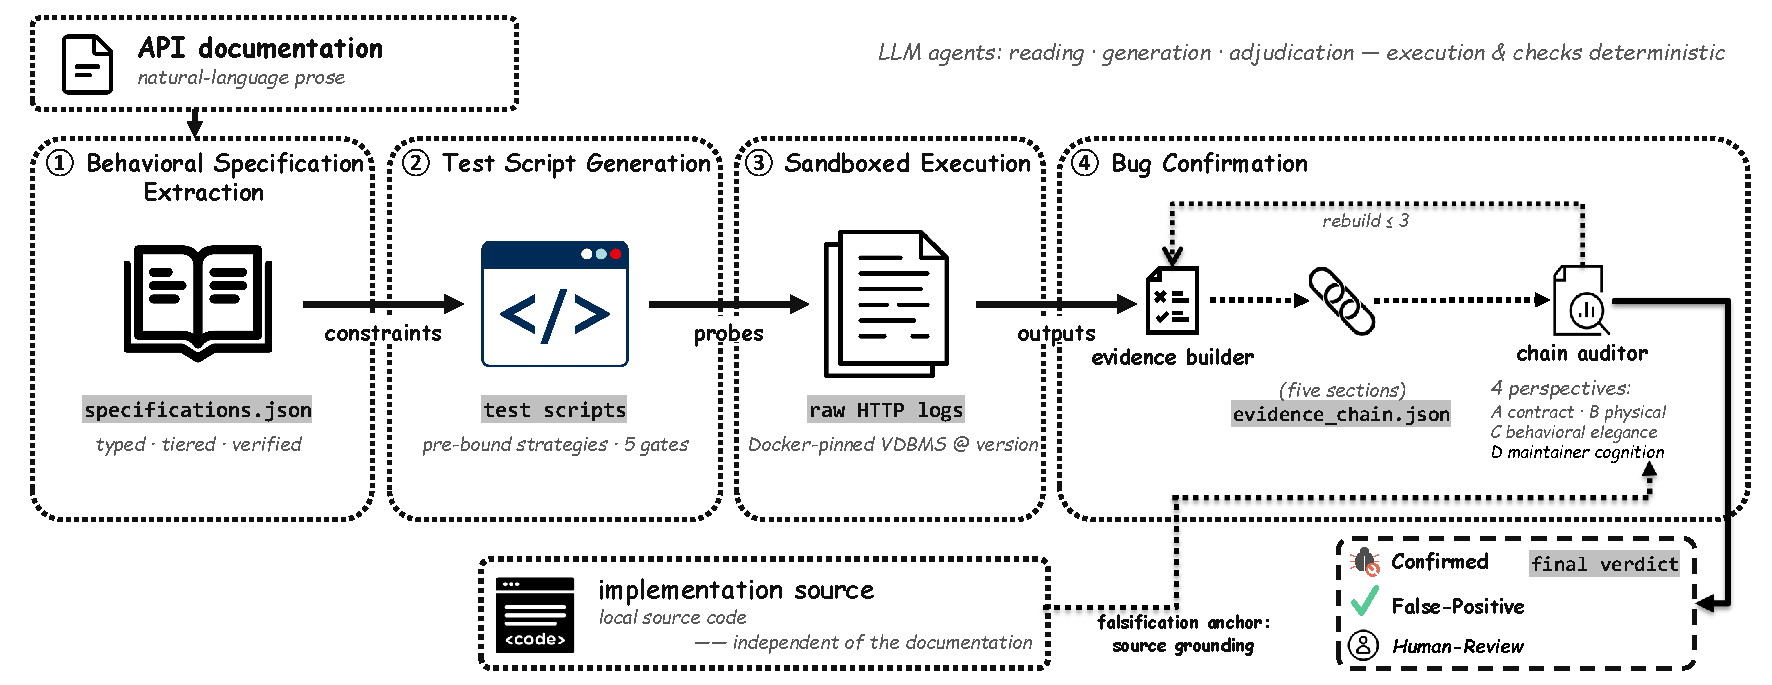
\includegraphics[width=0.76\linewidth]{figures/pipeline-v10}
\caption{\system{}'s four-stage pipeline. Stage~(iv) splits evidence assembly from cross-examination:
an evidence builder grounds each candidate in documentation, execution output, and implementation
source; a chain auditor applies four mechanical checks and then reads the chain from four
perspectives, under a fixed aggregation rule. Measured in this paper: the organization of stage~(iv)
and the evidence it is allowed to read.}
\label{fig:pipeline}
\end{figure}

Figure~\ref{fig:pipeline} shows the four stages. Two features make the design measurable rather than
merely usable: each stage writes a structured artifact---a constraint record, a probe with an inline
oracle line, a request/response log, an evidence chain---so a claim about a stage traces to the file
that grounds it; and the confirmation stage's evidence is \emph{frozen} per case, so every judge
configuration in Section~\ref{sec:eval} reads the same packages, and whatever it concludes it
concluded from the same material as the others.

Two real candidates run through the description. Milvus \#49823 documents \texttt{nprobe} as an
integer in $[1, 16384]$; the REST search API accepts \texttt{nprobe=0}, returns 200, and
answers---a boundary violation visible in one response. Qdrant \#10369 documents that a collection
referenced through \texttt{lookup\_from} must match the target's vector size; \texttt{recommend}
bypasses that check for negative examples and returns silently wrong scores, observable only after a
state transition. The two take different generation paths in stage~(ii), and both were confirmed by
maintainers.

\subsection{Behavioral-specification extraction}
\label{subsec:extraction}

\textbf{Knowledge extraction.} A \emph{knowledge extractor} crawls the vendor's documentation for
the target and its version and writes a per-endpoint knowledge file: method, path, source URL,
parameters, constraints, expected responses, plus a table tracking each page's documentation
version. Two self-checks gate the output---an endpoint-coverage check against the vendor's published
API surface, and a version-alignment check requiring the documentation version to match the
target's major.minor, because a specification read from the wrong documentation version tests the
wrong system. Version alignment is a precondition, not a post-hoc filter: where a crawled artifact
disagrees with the pinned version, the versioned documentation stays authoritative.

\textbf{Specification extraction.} A \emph{specification extractor} reads that file and emits one
record per constraint: a unique identifier, the endpoint, a natural-language description, a
checkable assertion (for \#49823's family, \texttt{nprobe >= 1 \&\& nprobe <= 16384}), a type, an
evidence tier, and a source URL with a verification flag. Three mechanisms discipline the model.
\emph{Categorization} types each constraint as range, type, state, behavioural or other, deciding
which attack agent owns it. \emph{Evidence tiering} records how directly the page supports the
constraint---verbatim, from an example, from behaviour, or convention---so test strength is graded
by its support. \emph{Source verification} fetches the cited page and confirms it carries the
asserted semantics; failures are marked and excluded from downstream reporting. A judge's package
also carries contract rows matched to the parameters a candidate probes and appended at rebuild, and
Section~\ref{sec:audit} audits every citation that reaches a package independently of this or any
earlier step.

\textbf{Two levels, decided observationally.} A constraint is endpoint-level or system-level by what
would prove a violation, not by how hard it is to construct: violated by a single request/response
pair is endpoint-level even where elaborate setup is needed, and violated only by relating
observations across requests or against evolved state is system-level. \#49823 is endpoint-level;
\#10369 is system-level, since the coupling it describes becomes visible only after a transition.

\subsection{Test-script generation}
\label{subsec:generation}

Three attack agents---boundary, state, and semantic---turn constraint records into executable Python
probes, each bound to strategies registered before generation with trigger conditions and oracle
templates. Boundary strategies probe at and beyond documented bounds, wrong JSON types, and the same
resource addressed through two key forms. State strategies build multi-request scenarios: partial
application of an operation the documentation describes as all-or-nothing, deletion concurrent with
use, and cross-object references left dangling by a transition. Semantic strategies check the
documented meaning of a response rather than its shape---a right status code with a misleading
message, or the accept/reject semantics of a documented parameter.

\emph{Strategy selection is not left to the model.} Strategies are bound to constraints
deterministically by a registry of (strategy, trigger predicate) entries matched against the
constraint's type, level and assertion surface; a constraint may trigger several and the agent
generates for each, and one that triggers none falls through to scenario construction. Because the
mapping is a function of the constraint record alone, the pairs are reproducible from the
specification file, and each probe carries an inline oracle line---a machine-checkable assertion
about the expected response---removing a degree of freedom in which the model could drift.

Generation splits on the constraint's level. An endpoint-level constraint with a bound strategy is
instantiated directly against its violation surface. A system-level constraint always goes through
scenario construction: the agent must first build the state in which the constraint binds, then
evaluate the assertion against that live state in both directions of any transition. For \#10369,
that means a size-4 lookup collection answering \texttt{recommend} with 200, then a delete and
recreate at size 8 after which the same request must be rejected with a dimension-mismatch error.

Every probe passes five gates before it may execute: it must compile; its constraint must exist in
the structured contract; it must avoid registered risky patterns (a request path with no safe
wrapper, a swallowed exception); it must not carry helper code fingerprinted to another vendor's
environment; and its oracle line must match the response shape the endpoint returns. Only passing
probes reach the sandbox; failures are regenerated.

\subsection{Sandboxed execution}
\label{subsec:execution}

An executor runs each passing probe from the host runtime against a Docker-pinned instance of the
target at the tested version---nothing but the database itself executes inside the container. Each
probe writes its raw request/response pair to a log and, only after the log is flushed, a completion
marker; per-batch marker counts are reconciled, so an interrupted batch is detectable and
re-runnable. The sandbox is what lets a candidate reproduce under a clean probe, and the raw records
are the behavioural evidence every later stage consumes. Section~\ref{sec:audit} describes what an
audit of that evidence found.

\subsection{Bug confirmation}
\label{subsec:confirmation}

The last stage decides whether a candidate is a defect. It is not a single judgment. An
\emph{evidence builder} assembles evidence and a \emph{chain auditor} cross-examines it, with an
explicit rebuild loop---a builder/judge split whose purpose is to keep the falsification separate
from the claim.

\textbf{Assembly.} The builder checks the observation against the specification, re-verifies the
citation independently of the extractor's own check, traces the chain \emph{contract $\rightarrow$
doc $\rightarrow$ script $\rightarrow$ log} and flags broken links. It then greps a clone of the
implementation \emph{at the pinned version}---the only authority for what the implementation
does---for the parameter and error-code keywords, follows the call chain, and records one outcome:
the promised validation is absent, present, by design in the source, unlocatable, or the search was
shallow. The result is a five-section chain---document verification, execution evidence, contract
grounding, chain trace, source grounding---each labelled with the kind of evidence it rests on.

\textbf{Cross-examination.} The auditor applies four mechanical checks: all five sections non-empty;
contract, documentation, log and source agreeing; no internal contradiction; and the primary
observation matching the specification. A chain that fails goes back for rebuild, at most three
times. Surviving chains are then read from four
perspectives:

\begin{itemize}
  \item \textbf{A --- contract.} Does the quoted contract text actually ground the assertion? Run as
    a mechanical containment check.
  \item \textbf{B --- objective constraints.} Seven classes that constitute violations without any
    contract endorsement: numeric lower bounds on count-, size- and limit-class parameters, closed
    enum sets, mutually exclusive parameters, type tautologies, same-family inconsistency, interface
    asymmetry across a system's REST, gRPC and SDK faces, and (heavily qualified) HTTP response
    semantics. An \texttt{ef}/\texttt{nprobe}-class carve-out applies where the source documents a
    negative-sentinel convention.
  \item \textbf{C --- behavioural elegance.} May the implementation refuse the bug reading? Only an
    \emph{explicit} by-design may refute: the excerpt must carry intent evidence---a comment or
    docstring---or a maintainer quote must declare the class intended. Bare structural inference
    (``no validation is present'') is a weak refutation, routed to human review rather than closing
    the case. This is the clause Section~\ref{sec:census} audits.
  \item \textbf{D --- maintainer cognition.} Does a corpus distilled from the target's historical
    issues and merged PRs support either reading? Hits must match at the level of phenomenon, never
    by word overlap. Cognition states a maintainer's attitude; it may decide a contract-neutral case
    but may not supply a missing observation.
\end{itemize}

\textbf{Aggregation, and the verdict space.} The verdict is three-valued: Confirmed,
False-Positive, or Human-Review. Aggregation is fixed, and the order in which its clauses are tried
is part of the design: a contract confirmation decides the case; a contract refutation \emph{with}
the objective-constraint perspective confirmed routes rather than closing; otherwise a contract
refutation closes to False-Positive; an objective-constraint confirmation decides a
contract-neutral case; a cognition hit on either side decides a case the earlier clauses left open;
an explicit by-design refutation closes; everything else routes. The order is not a
detail---\textbf{the clause that closes a judgment is the first in this sequence that decides
it}, which is exactly what Section~\ref{sec:census} counts. The rule is deliberately
asymmetric---only explicit intent evidence may refute, and anything unsettled goes to a
person---a design position rather than a claim of
precision. An LLM-derived oracle is expected to over-report; the protocol keeps the over-reporting
visible in a review queue instead of suppressing it at the cost of discarding real defects.
Section~\ref{sec:eval} measures what the asymmetry costs and what it buys, and
Section~\ref{sec:census} shows where the errors it does not catch actually land.

\textbf{Implementation.} The pipeline runs as a multi-agent system on an agentic coding runtime, one
role prompt per agent, all agents on a single model backbone under vendor-default sampling. Each
stage's artifact is versioned, and the Section~\ref{sec:eval} study reads frozen copies of them
rather than re-running the pipeline.

\section{Evaluation}
\label{sec:eval}

We evaluate on 81 adjudicated cases from three production VDBMSs, under one frozen set of packages
(Section~\ref{sec:method}), to answer three questions.

\begin{itemize}
  \item \textbf{RQ1:} What does the campaign yield, and on what does it rest?
  \item \textbf{RQ2:} How much of what the confirmation stage reads is actually in the documentation?
  \item \textbf{RQ3:} Where does the confirmation stage's error come from?
\end{itemize}

\subsection{Methodology}
\label{sec:method}

\textbf{The pool.} Eighty-one candidates from Milvus, Qdrant, and Weaviate: 51 maintainer-confirmed
bugs and 30 adjudicated false positives. Ground truth is maintainer adjudication for the 51 (labels,
closures, merged fix PRs); the 30 negatives are adjudicated by us against the maintainers'
disposition where available---the ledger's basis groups \textbf{eleven of the thirty}, and the
vendors' own \texttt{resolution/by-design} labels a further twelve, a label reporters cannot apply
and Milvus maintainers set per issue: \textbf{at least twenty-three carry a maintainer disposition},
at most seven are our own calls. There is no inter-annotator study. The shipped ledger holds 132
rows: 81 adjudicated and 51 unadjudicated, of which 49 carry no maintainer verdict and 2 are our own
withdrawn submissions. \textbf{One of the 81, \texttt{milvus\_001}, is
unjudgeable}---its observation was never captured and its version's documentation segment is
retired. Under the deployment's convention, which credits a routed case, \textbf{eleven of the
twelve configurations route it to Human-Review in at least two of their three runs}---only the
contract core never does---so eleven are \textbf{credited a point for a case nobody could judge};
under the forced and joint readings it is a guaranteed miss.

\textbf{What the screening does not move.} The reported run registered \textbf{32 further candidates,
screened out before submission}; re-adjudicated under the same protocol minus the cognition
perspective (whose corpus could carry maintainer verdicts for their families), three runs each, the
stage confirms \textbf{19 of 32 (0.594)} where the deployed stage, which does read that perspective,
confirms \textbf{48 of 81 (0.593)} on the pool---so the two rates are not one instrument's. The 32
have no maintainer ground truth: this bounds the submission filter, and does not separate the
streams.

\textbf{Two leak repairs, and why they are load-bearing.} The same audit
exposed two channels through which material the confirmation stage was forbidden to read had reached
it. First, \textbf{ten of the 81 rebuilt packages carried an embedded maintainer-cognition
section}, which the core, flat and source-only dispatches forbid; it was stripped and all ten cases
re-judged, spanning \textbf{five configurations}---contract core, flat judge and source-only on the
primary at three runs each, the second backbone's source-only at three and its flat judge at one,
that arm's other two runs having been dispatched after the strip. Second, \textbf{the runtime
cognition files referenced seven of the 81 candidates' own issue numbers}; the entries were removed
and those seven cases re-judged. That repair reached the deployed stage on both backbones but, we
found later, \textbf{not the two full-family controls}, whose recorded rationales still cite the
removed entries by issue number; those six runs have since been re-judged on the same terms.
\textbf{Every number this paper reports is computed on the cleaned pool}, and the second repair is
not cosmetic: without it the deployed configuration would read 41/51 with a confirmed set of 41+6
rather than the 39/51 and 39+9 we report. It does not move the two controls in our favour either: of
the nineteen verdicts the six re-judge files rewrite, fifteen move a case toward confirmation under
the convention and four between Confirmed and Human-Review, which the convention counts alike, so
none moves away; the arms' true-positive sets are unchanged (48 and 33) while the false positives
they leak rise by two and one---suppression, the share of the 30 negatives an arm does not confirm,
falls $0.467\to0.400$ and $0.933\to0.900$; on the forced reading the no-source arm gains one, to 31.
Both raw generations ship alongside the cleaned one.

\textbf{The counting convention, and its price.} A verdict is Confirmed, False-Positive, or
Human-Review; Human-Review is the deployment's escalation channel. We count a routed case as
confirmed, because that is what the deployment's ledger counts---and the convention is not free,
because a configuration that routes more scores higher on recall. So we report the forced-verdict
reading beside it for every contrast, and we price the convention at \textbf{two} places: the arms'
levels, and the headline contrast itself. The rulings come from one author-executed non-blind pass;
an independent adjudicator on the same materials agrees with it on 4, 5 and 6 of the 20 commonly
ruled cases under the pack-only, pack-plus-source and full-protocol statements respectively
($\kappa = -0.01$, $0.08$, $0.11$), so we report the joint reading as a bound rather than a
measurement. \textbf{Two of the three independent passes land at the forced floor.}

\textbf{The twelve configurations.} Each re-adjudicates all 81 cases three times. A case counts as
confirmed when \textbf{at least two of its three runs recorded it as confirmed}---under the
convention, either Confirmed or Human-Review---which is not the same as requiring two runs to agree:
three cases split three ways, and under that stricter rule the deployed stage would recall 37/51
rather than 39/51. Both backbones are serving aliases without pinned weights; \textbf{the primary is
GLM-5.3-Flash and the second Qwen3.8-Flash}, and Table~\ref{tab:configs} lists the twelve.

\begin{table}[t]
\caption{The twelve judge configurations. Each re-adjudicates all 81 cases three times; only what
the judge is given and which rules it applies differ.}
\label{tab:configs}
\footnotesize
\begin{tabular}{@{}rlcccl@{}}
\toprule
\# & configuration & perspectives & rule & source & backbone \\
\midrule
1 & contract core & --- & --- & --- & GLM-5.3-Flash \\
2 & flat judge & --- & --- & $\bullet$ & GLM-5.3-Flash \\
3 & flat $+$ schema fix & --- & --- & $\bullet$ & GLM-5.3-Flash \\
4 & flat $+$ aggregation & --- & $\bullet$ & $\bullet$ & GLM-5.3-Flash \\
5 & full, no aggregation & $\bullet$ & --- & $\bullet$ & GLM-5.3-Flash \\
6 & source-only & --- & --- & $\bullet$ & GLM-5.3-Flash \\
7 & full stage & $\bullet$ & $\bullet$ & $\bullet$ & GLM-5.3-Flash \\
8 & full, no source & $\bullet$ & $\bullet$ & --- & GLM-5.3-Flash \\
9 & flat judge & --- & --- & $\bullet$ & Qwen3.8-Flash \\
10 & flat $+$ aggregation & --- & $\bullet$ & $\bullet$ & Qwen3.8-Flash \\
11 & source-only & --- & --- & $\bullet$ & Qwen3.8-Flash \\
12 & full stage & $\bullet$ & $\bullet$ & $\bullet$ & Qwen3.8-Flash \\
\bottomrule
\end{tabular}
\end{table}

We added them during the study rather than pre-registering them, and \textbf{three contrasts change
more than one thing}: contract-core-to-flat (any judgment at all, against a binary-only core), the
deployed change (verdict space plus routing rule, decomposable only on the primary backbone), and
the four-perspective contrast (five things, listed in Section~\ref{sec:buys}).

Each control is a traceable edit of the arm it extends. The schema-fix arm changes only the flat
dispatch's output-schema line, from a binary to a three-valued \texttt{verdict} field. The
aggregation arm changes that same line, the sentence declaring that no aggregation rule applies, and
appends the routing clause. The source-withheld arm drops the \texttt{source=} path from every
per-case material line of the full-stage dispatch. The no-aggregation arm excises both aggregation
blocks. The flat judge is the full stage's materials without the perspective vocabulary and the
aggregation rule, and it keeps the protocol's red lines---the verbatim-intent requirement for
by-design refutation, and the objective-constraint principle stated with four of its seven classes
as examples rather than the full enumeration. Every judge received the same per-case materials---its
frozen evidence pack and that case's version-pinned source clone---under identical discipline
clauses: its own pack and clone only, no network access, cases judged independently. All dispatch
texts ship verbatim in the artifact, with English renderings of the two judging prompts (the
full-stage protocol and the flat judge's) under \texttt{rq2/prompts/}.

\textbf{A defect we report rather than repair.} Eight of the twelve dispatches declare a binary
\texttt{verdict} field while their own text mandates three values. It is part of the baseline on
those eight; the declared field was not binding in practice---the flat judge recorded Human-Review on
21 of 243 judgments against a binary schema.

\textbf{Statistics.} Paired exact McNemar at both the confirmed-set level (81 cases) and the recall
level (51 true bugs); they disagree and \textbf{both are reported for every contrast}, including the
isolation steps. Matched-pairs Wald intervals on recall differences. Discordant pairs are written
\emph{a/b}, where \emph{a} is the arm whose count is printed first in the comparison being reported.
\textbf{The p-values we print are unadjusted.} Twenty paired tests appear below, ten of them at the
recall level; the family is those ten because they share a pool (the 51 true bugs), which the confirmed-set tests
do not. Read as a family of ten, a Holm correction leaves the four smallest significant---the
bundled contrast on the second backbone ($0.0001$), that backbone's perspective contrast
($0.0034$), the bundled contrast on the primary backbone ($0.0039$) and the evidence-access contrast
($0.0039$), tested against $\alpha/10$, $\alpha/9$, $\alpha/8$ and $\alpha/7$---and stops at the
fifth ($0.0225$), so the deployed stage's own recall-level advantage over the flat judge, and
everything larger than it, should be read descriptively. \textbf{The family choice is load-bearing,
so we report it both ways}: read instead as the twenty printed tests, seven clear their step-down
thresholds and the sequence stops at the first $0.0039$, so the two $0.0039$ contrasts also fall to
descriptive---while the second backbone's perspective contrast at $0.0034$ survives either family. All rates, the census on both backbones,
both replays, the net and $F_1$ intervals and the pair audit are recomputable from the artifact's
five analysis scripts, all under \texttt{rq2/analyses/}: \texttt{recompute\_paper\_numbers.py},
\texttt{clause\_tally.py}, \texttt{convention\_pricing.py}, \texttt{bootstrap\_net\_f1.py} and
\texttt{audit/pair\_audit.py} --- with \texttt{clause\_tally.py second} giving the second backbone's
census and running the letter-identification test, and the guard price replayed from the audited
closure reading the package ships. The catch-all composition, the expectation-framing check and the
C row's evidence classification are printed but not yet scripted, and the artifact's coverage note
says so.

\subsection{Mining yield (RQ1)}
\label{sec:yield}

Maintainers confirmed 51 of the 81 adjudicated submissions; 23 are fixed by merged PRs. The 51 break
down as 23 fixed, 18 acknowledged-open, 7 closed without a fix, and 3 tracked as duplicates. Per
system: Milvus 43 adjudicated (29 confirmed / 11 fixed / 14 false positives), Qdrant 28 (14 / 9 /
14), Weaviate 10 (8 / 3 / 2). One of the 51 is a crash-or-panic defect; the other 50 are silent
accepts, wrong results, or poor diagnostics. A separate analysis in our development tree records
that all 23 merged fixes modify implementation code, 15 also add a regression test, and none is
documentation-only; \textbf{that table is not part of the shipped artifact and we mark the claim
accordingly}.

\textbf{Attribution, and what was voided.} The ledger records 132 rows across 19 versions of the
three systems; the 81 adjudicated submissions span 16 of those versions and the 51 confirmed bugs
span 15. It is \textbf{not a per-run detection rate, and we cannot supply one}: the
\emph{detection-ability} experiment---15 versions run to measure per-version detection---was
\textbf{voided in full on 2026-08-23} because its attack dispatches carried source-clone paths and
cross-round experience, violating our own information-boundary rules, with quality gates missed on
the versions that were clean. Those runs measure nothing. \textbf{A substantial share of the 81
adjudicated submissions sits on versions that experiment covered}, so the distinction matters and we
state it: the voided object is the \emph{measurement}, and the adjudication survives because
maintainers are external to the violated protocol---they confirmed the candidates and merged the
fixes. We report the ledger for that reason and no other. The void record ships with the artifact.

\subsection{Auditing the evidence packages (RQ2)}
\label{sec:audit}

The stage reads a per-case package: the candidate's observation, and constraint rows distilled from
vendor documentation with a citation on each. We audited every cited pair against the page it cites,
at the version the row claims, \textbf{on the packages as the pipeline produced them}: the rebuild
below follows this audit, so the split describes the material as found rather than the material the
judges went on to read.

\textbf{Pair level: 134 (constraint, cited-page) pairs}, deduplicated from the surviving row
instances; Table~\ref{tab:pairaudit} gives the three-way split.

\begin{table}[t]
\caption{The pair-level audit. The two 43.3\% shares are each of 134, not a combined 86.6\%.}
\label{tab:pairaudit}
\footnotesize
\begin{tabular}{@{}lp{0.57\textwidth}@{}}
\toprule
Verdict & meaning \\
\midrule
supported as cited \textbf{(18, 13.4\%)} & the cited page documents the constraint \\
re-anchored \textbf{(58, 43.3\%)} & the cited anchor was a \emph{source file} (a
\texttt{constant.go} path) or an \emph{API landing page} carrying no endpoint documentation; the
constraint was re-anchored to version-pinned documentation or the pinned API specification \\
no support on the cited page \textbf{(58, 43.3\%)} & the cited page does not support the constraint,
and for many no page does \\
\bottomrule
\end{tabular}
\end{table}

\textbf{Case level: 12 main assertions}---a different object, the case's own headline claim rather
than its citations. Five were supported (recorded by quoting the page verbatim, or---for three cases
whose assertion was the same schema-match sentence---by replaying the observation against the
operator's page), \textbf{three were dropped as unsupported} (no constraint entry on the pages
checked), \textbf{two were over-strong} and were respectively rewritten to the page's own claim and
weakened to a descriptive statement, and two were recorded as weak-evidence rows with the page's own
normative-free wording. All twelve were acted on.

\textbf{The two dominant mechanisms.} \emph{Version drift}: the augmentation script drew every
vendor's constraints from one fixed version's contract, so rows for one release carried another
release's endpoints and shapes. \emph{Conceptual-only documentation}: constraints such as
\texttt{nprobe} $\in [1, \texttt{nlist}]$, \texttt{M} $\in [4, 64]$ or a password length bound exist
as prose descriptions but not as documented values, so a distiller that states them asserts more
than the page does.

Every package was then rebuilt against version-pinned documentation and all rows re-anchored, and we
checked the rebuilt set for the failure this class of work invites: \textbf{zero of 81 packages
contain a sentence framed as an expectation}---the 19 hits for such phrasing were each inspected and
are all verbatim server responses, quoted as observations.

\textbf{What it means.} This measures a step every ``distil a specification from documentation, then
judge against it'' pipeline performs and that, to our knowledge, none reports. \textbf{We are not
claiming these rates as properties of LLM distillation in general}---they are this distiller on
these three vendors' documentation---but they
are high enough that the next pipeline in this line should measure its own numbers before
attributing a confirmation rate to its judge. \textbf{A blind second reader on a stratified sample
of 36 of the 122 pairs whose cited page is still reachable agrees on 30 (\textbf{$\kappa = 0.75$})}:
all 12 SWAP pairs were called SWAP again, and the six disagreements are three at the DROP/SWAP
boundary and three at SUPPORTED/DROP.

\subsection{What the confirmation stage buys}
\label{sec:buys}

This section supplies the instrument; Section~\ref{sec:census} carries the paper's claim.

\textbf{Levels.} At its deployed configuration the stage confirms 39 of 51 true bugs and intercepts
21 of 30 false positives under the deployment's convention; forced, 27/51 at suppression 27/30;
under the hand-adjudicated joint reading, 33/51. The contract-only core suppresses 29/30 but recalls
8/51; the no-aggregation arm confirms 33 with 3 leaked false positives (suppression 0.900, precision
0.917).

\textbf{The headline contrast, priced.} The flat judge differs from the deployed stage in several
things, so we added the missing pieces to the flat judge in turn. The schema-line repair alone moves
recall 30$\to$35 (recall level 0/5, $p{=}0.0625$; confirmed-set level 34$\to$39, 1/6,
$p{=}0.1250$) and forced recall 25$\to$29; adding the routing rule on top moves recall 35$\to$39 at
the recall level (2/6, $p{=}0.2891$; confirmed-set 39$\to$51, 2/14, $p{=}0.0042$) and, forced, the
other way (29$\to$27, 3/1). \textbf{The bundled contrast---flat judge to rule-bearing judge---moves
30$\to$39} at the recall level (0/9, $p{=}0.0039$) and 34$\to$51 on the confirmed set (0/17,
$p{<}0.0001$), and it replicates on the second backbone: 27$\to$41 at the recall level (0/14,
$p{=}0.0001$) and 32$\to$51 on the confirmed set (0/19, $p{<}0.0001$). \textbf{The two levels
disagree for the rule step, and we privilege neither}: it is significant at the confirmed-set level
and not at the recall level. For reference, the deployed stage against the flat judge is 48 vs 34 on
the confirmed set (16/2, $p{=}0.0013$) and 39 vs 30 at recall (11/2, $p{=}0.0225$).

\textbf{Under our own hand-priced reading the change is worth three, and that is a floor.} Applying
the same hand-adjudication of the routed queue to this contrast gives the \textbf{rule-bearing
control}---which is not the deployed stage---32/51 against the flat judge's 29: \textbf{+3}. The
deployed stage itself is 33/51 against the same 29---\textbf{+4}. The control's routed queue holds 25
cases---a case is in it when at least one of its three runs records Human-Review and its majority is
confirmed---of which 9 were never ruled, one of them a true bug; the flat judge's holds 11, of which
2 were never ruled, none a true bug. Crediting every unruled case on \textbf{both} arms symmetrically gives
33 against 29---\textbf{+4}; crediting the control's unruled \emph{and} return-ruled cases while
leaving the flat judge strict gives +5. \textbf{At the reading this paper considers honest, the
deployed change is suggested, not established}, and on the second backbone there is no
schema-repaired control, so the split is unmeasured there.

\textbf{The four-perspective contrast.} It changes \textbf{five things} against the rule-bearing
flat judge: the perspectives; the aggregation rule text, since a perspective-free judge cannot carry
an A/B/C/D clause table; the red-line set; the declared verdict field; and access to the cognition
corpus. With that label: 39 vs.\ 39 on the primary backbone (4/4, $p{=}1.0$; interval $\pm0.11$, so
the data exclude an effect larger than about eleven points but do not establish equivalence), and
\textbf{$-11$ true bugs on the second} (41 vs.\ 30, 12/1, $p{=}0.0034$); on the confirmed set the
same two are 51 vs.\ 48 (9/6, $p{=}0.6072$) and 51 vs.\ 35 (18/2, $p{=}0.0004$). Under forced verdicts the
two are equal on both backbones (27 vs.\ 27; 26 vs.\ 26); equal, but not the same decisions---their
forced true-bug sets intersect in 22 of 27 and 23 of 26. At the recall level against the rule-free
flat judge the perspectives are $+3$ (33 vs.\ 30, 5/2, $p{=}0.4531$) and against the
schema-corrected control $-2$ (33 vs.\ 35, 1/3, $p{=}0.6250$), neither significant; on the confirmed
set those two are 36 vs.\ 34 (6/4, $p{=}0.7539$) and 36 vs.\ 39 (2/5, $p{=}0.4531$).

\textbf{The readings reorder the arms.} Across the nine judging arms this section contrasts---the
flat judge, flat $+$ schema, flat $+$ aggregation, full-no-aggregation, full stage and full-no-source
on the primary backbone, and the second backbone's flat, flat $+$ aggregation and full---forced
recall spans [23, 31] of 51 against a convention span of [27, 48]; the contract-only core, a blind
baseline, reaches 8 forced and 8 convention, and the two source-only configurations 20 and 19 forced
(36 and 37 convention, the two recall figures quoted below).

\textbf{What evidence access costs.} Withholding the implementation source raises recall
39$\to$48 (discordant 0/9 at the recall level, $p{=}0.0039$; forced 27$\to$31) and cuts suppression
from 21/30 to 12/30, so it buys nine true bugs and releases nine more false positives. On the
confirmed set the same contrast is 48 vs 66 (discordant 0/18, $p{<}0.0001$). \textbf{The deployment's
summary metrics do not separate the two configurations}: net true positives minus leaked false
positives is 30 either way---a difference of 0, paired case-level bootstrap 95\% CI $[-8,+8]$---and
$F_1$ is 0.821 without the source against 0.788 with it, a difference of $+0.033$ whose interval also
spans zero ($[-0.044,+0.115]$). A configuration that drops its most trusted evidence channel
therefore matches the deployed stage on net and is not separated from it on $F_1$ either---the price
of the falsification anchor, stated as a tie rather than as a defeat. Two caveats: the arm is not
source-access-only (it also redirects the by-design clause to the cognition materials and drops the
objective-constraint perspective's negative-sentinel exemption), and the two source-only
configurations (0.706 and 0.725 recall) are shipped but outside this section's contrasts.

\subsection{The clause census (RQ3)}
\label{sec:census}

The census covers \textbf{the deployed stage on the primary backbone}---81 cases, three runs each,
243 judgments. We state the scope because it is narrower than the claim sounds and because we can
check it: the same census on the second backbone does not reproduce the pattern. There, contract
refutation closes 56 judgments and by-design refutation closes 50, of which 22 are wrong---so
by-design is not the accurate clause on that backbone---and the unguarded clause supplies 24 of 48
incorrect closures to False-Positive, \textbf{50\% rather than 80\%}. That comparison is itself
bounded in one place. The content test run there---only C records a weak refutation (11 cells), only
D carries the source vocabulary---passes as it does here, so the letters are not swapped between
backbones. What is not settled is what D \emph{means}: the dispatch defines the four perspectives
twice with C and D exchanged (defect 3) and its schema follows the first definition for D and the
second for C, so D's cells carry two incompatible vocabularies---the source one in \textbf{217 of 243
judgments there against 98 here}, the cognition one in the remainder---and the aggregation's D
clauses, which key on the cognition values, fire \textbf{twice against 23}. The reversal above is in
C, which is identified on both backbones, not in D, whose content is not.

\textbf{On the primary backbone the letters are identified by their content rather than assumed.}
Every recorded cell carries a value from that perspective's legend, and two of the four are
identified uniquely: no cell outside C records a \emph{weak} refutation (C is Confirmed 72, Neutral
71, Weak-Refuted 59, Refuted 41), and no cell outside D carries the source vocabulary. A and B share
three values but not their shape: A is Neutral 172, Refuted 50, Confirmed 21; B is Neutral 146,
Confirmed 80, Refuted 17---which they do not need: the dispatch names A and B the same way in both
definitions, so they are what their field names say; C and D are the pair it names twice with the
definitions exchanged. The nineteen judgments this census
closes by C=Refuted record what they rest on, and reading them
separates three kinds of evidence rather than one: \textbf{fifteen} cite a comment or docstring in
the implementation; \textbf{two} (\texttt{milvus\_026}, in two of its three runs) cite the server's
own name-validation rule, whose code and error message those runs name; and \textbf{two}
(\texttt{milvus\_011} and \texttt{milvus\_012}, each in its third run) rest on code structure---a
default expression, a fallback chain. None rests on observed behaviour alone---but the legend asks
for more than that, \textbf{affirmative} intent evidence in a comment, docstring or maintainer
quote, and the last two do not clear it. The same two cases
show why the distinction is not academic: in both, the case's \emph{other} runs recorded a weak
refutation and gave their reason---\texttt{milvus\_011}'s second run notes that a silent behaviour
has no comment behind it, and \texttt{milvus\_012}'s second run states that the fallback-chain
structure shows design but carries no comment or quote, so the red line governing this perspective
does not admit it. The verbatim-evidence requirement is therefore not applied uniformly by the judge
that recorded these cells---a departure the compliance recount below does not catch, because that
recount measures compliance with the \emph{aggregation} rule, and this is a requirement of the
perspective itself. The primary's D cells likewise carry the cognition vocabulary in 145 of 243
judgments against the source vocabulary's 98, which is the split that puts the latter in the
catch-all below. The ambiguity between the two printed definitions therefore bounds the cross-backbone
comparison without voiding the census on the backbone we claim. What we claim is the primary-backbone
result; what we can say about the second is that it does not reproduce and that we cannot rule out
the letters meaning different things there.

The clause legend, in firing order: \textbf{A} the contract perspective (Confirmed, or Refuted where
the contract assertion is contradicted, with the exception that Refuted plus B Confirmed routes);
\textbf{B} the objective-constraint perspective; \textbf{D} maintainer cognition; \textbf{C}
behavioural elegance, refuting only on verbatim intent evidence---an in-source comment or docstring,
or a maintainer quote; then the catch-all. ``Accuracy'' is agreement with the maintainers'
adjudication. Table~\ref{tab:census} is grouped by the outcome each clause assigns.

\begin{table}[t]
\caption{The clause census over the deployed stage's 243 judgments on the primary backbone.}
\label{tab:census}
\footnotesize
\begin{tabular}{@{}llrrrr@{}}
\toprule
Clause & assigns & n & right & wrong & accuracy \\
\midrule
B = Confirmed & Confirmed & 61 & 56 & 5 & \textbf{0.92} \\
A = Confirmed & Confirmed & 21 & 17 & 4 & 0.81 \\
D = Supports-Defect & Confirmed & 7 & 5 & 2 & 0.71 \\
\textbf{A = Refuted} & False-Positive & \textbf{50} & 26 & \textbf{24} & \textbf{0.52} \\
\textbf{C = Refuted} & False-Positive & 19 & 17 & 2 & \textbf{0.89} \\
D = Supports-Not-Defect & False-Positive & 16 & 12 & 4 & 0.75 \\
catch-all & \textbf{Human-Review} & 69 & \emph{45 bugs} & \emph{24 FPs} & --- \\
\bottomrule
\end{tabular}
\end{table}

\textbf{The protocol guards the clause that is already clean.} By-design refutation must rest on
verbatim intent evidence and perspective C enforces that. C is the most accurate refuting clause
measured (17 of 19) and the least often fired of the two refuting clauses---\textbf{the middle of
the three clauses that assign False-Positive} (19 judgments, against cognition's 16 and contract
refutation's 50); it closes 2 of the 243 judgments that rest on true bugs. Contract refutation
carries no such requirement, closes two and a half times as many, and is wrong about half the time:
\textbf{24 of its 50 closures fall on confirmed bugs, and of the stage's 30 incorrect closures to
False-Positive this one clause supplies 24---80\%}. \textbf{This is not the pair audit's finding
resurfacing.} The clause is a mechanical containment check, and the audit found 58 of the 134 cited
pairs unsupported, so the two results could be one phenomenon---defective rows failing a containment
check rather than a protocol closing wrong---in which case the prescription would be to fix the
material rather than to guard the clause. The cross-tab separates them. Over the 81 packages' four
strata: of the 24, \textbf{20 fall on the 59 cases whose rebuilt packages carry documented evidence}
(20 of their 177 judgments, rate 0.11), 4 on the 3 weak-evidence packages, and \textbf{none on the
eighteen the audit left without documented evidence} (rate 0.00) or on the eighty-first, whose
observation replay is incomplete. The strata are a different object from the twelve assertion-level
rows of Section~\ref{sec:audit}. The clause fires on material the audit judged
supported. \textbf{A second rival is selection.} Contract refutation is tried before the by-design
perspective, so it fires on the largest and most heterogeneous set, while C = Refuted closes only
the 19 that A, B and D all left open; the accuracy gap (0.52 against 0.89) is therefore consistent
both with the guard working and with C's residual being the easier set. The prescription does not
need that resolved, because it rests on \textbf{error mass}---50 closures wrong 48\% of the time is
24 errors, against 19 wrong 11\% of the time is 2---and a guard belongs wherever the errors are.
Three facts make this count the census's most
robust, all of them about how it is constructed rather than how far it travels---the scope above
bounds the latter---with one disclosure: the counts above are post-repair, and the archived
pre-repair cells would give contract refutation 47 closures and by-design 20, so ``by-design is the
middle of the three'' holds of the cleaned pool. The load-bearing 24 is invariant either way.
\textbf{It is invariant across the two aggregation rules our dispatch prints}, whose last steps
disagree about the insufficient-evidence default, because contract refutation assigns
False-Positive under both---and no recorded cell \textbf{on this backbone} carries the
A=Refuted-with-B=Confirmed pair that the other rule would route (the second backbone records three).
\textbf{Its load-bearing count is computed on maintainer-confirmed labels} (the 24 closures that
fall on true bugs), so it does not rest on the 30 negatives. And it
survives the two leak repairs above, which were applied before these judgments were recorded.

\textbf{The counterfactual, at both readings.} Routing contract refutation to human review,
everything else held at the recorded perspective values, moves recall 39/51 $\to$ \textbf{46/51} and
suppression 21/30 $\to$ \textbf{12/30} under the convention---seven true bugs gained and nine more
false positives released, since a routed case is confirmed rather than judged; \textbf{forced, the
same replay changes nothing} (27/51, 27/30, identical sets), because an abstention and a closure score
the same there. Fifteen cases are closed by the clause in two or more of three runs, seven of them
true bugs and all seven unconfirmed---\textbf{seven is the case-level maximum on the bug side}; one
further negative closes in a single run. \textbf{The guard prices the same.} The prescription is a
guard, not a routing rule, so we read the fifty closures on the axis the by-design clause is held to:
\textbf{forty-two cite neither} an in-source comment or docstring nor a maintainer quote (the eight
that do are five runs of one docstring and three others), and routing those 42 leaves \textbf{the same
confirmed set}, because every case the clause touches closes in two or more runs and clears in
one---so the replay is not a loose upper bound but the guard's own price, and that price is still one
the convention sets rather than the stage's decisions.

\textbf{The escalation channel, restricted to the cells the rule defines.} The catch-all routes 69
judgments. \textbf{Thirty-seven (54\%) carry the source vocabulary in their D cell}---which the
operative rule has no clause for, so they fall through by classification rather than by the judge's
reasoning; those 37 rest on 28 true bugs. Of the \textbf{32 whose D cell uses the cognition
vocabulary}---all \texttt{NO\_SIGNAL}, which the aggregation also has no clause for---\textbf{17 rest
on true bugs (53.1\%)} against a pool base rate of 63.0\%, about one standard error below it, so we
could not detect enrichment. The honest reading is the composition, not a rate.

\textbf{The judge departs from the appended rule in 22 of 243 judgments forward and one in
reverse}---17 forced to False-Positive, which the red lines forbid, and 5 to Confirmed; \textbf{10
of the 17 rest on true bugs}. Replaying with the rule enforced moves 39/51 $\to$ 43/51 and 21/30
$\to$ 19/30 under the convention, and nothing under the forced reading. One caveat bounds the
paragraph: the dispatch prints an earlier rule whose last step commands exactly those closures, so
they are deviations from the appended rule and compliance with the earlier one.

\subsection{Comparison with the crash-oracle baseline}
\label{sec:baseline}

Run to natural completion against the Qdrant instance where our silent-accept defects are live, the
released VDBFuzz template set (205 templates; 50.8 minutes; the per-template logs record every
mutation loop and every response) produces \textbf{0 oracle anomalies}. Those logs record 1,127
mutation stages and 11,629 response-status lines with no 5xx anywhere; the runner's master log is a
verbatim echo of them, so a total taken over the shipped directory doubles, and we report the
single-copy figures. The oracle fires on 5xx rather than on service death, and the released mutation
vocabulary tops out below the values some crash classes need, so the zero bounds \textbf{the released
configuration's} reach into the silent majority, not the crash-oracle family. A hand-guided probe
built on the pipeline's boundary reasoning submits a value that vocabulary cannot reach; the script
ships and its output was not retained, so no execution result is claimed.

One artifact meets a reader who opens the logs to audit the zero: across 119 of the 205 per-template
logs, 152 single-copy lines each report three anomalies, from the baseline's own no-mutable-fields
path returning a three-key dictionary where its caller counts failures. They are not oracle
decisions---every stage-completion line records zero---but they look like anomaly reports, and we say
so rather than leave them to be found.

\section{Discussion}
\label{sec:discussion}

\textbf{Audit what your oracle reads, not only what it concludes.} Thirteen per cent of the
constraint-page pairs our stage read were supported by the page they cited; another 43\% cited the
wrong kind of anchor, and 43\% had no support at all. Every pipeline in this line distils
documentation and judges against the distillation, and the distillation is the step nobody measures.
It is cheap to measure: a sample of pairs against their cited pages tells you how much of your
judge's input is unsupported, and crossing that against where its errors land---the test
Section~\ref{sec:census} runs---is what settles whether the rate is a property of the judge or of
the materials.

\textbf{Put the evidence guard where the error mass is.} On the deployment we audited, the protocol
requires verbatim intent evidence for the refutation it makes least often and gets most right, and
requires nothing for the one that closes the most judgments to False-Positive and is wrong half the
time. The counterfactual prices the fix at seven true bugs gained and nine false positives released
under the convention, and at nothing under the forced reading---the cleanest demonstration that it is
the convention, not the judge, that pays for abstention. The prescription is bounded by what we
measured: the error mass moved on the second backbone, where the guarded clause closes 50 and is
wrong 22, so the rule is advice about where to look rather than a property of the protocol.

\textbf{Price the deferral channel, and price the contrast, not just the level.} The routing change
(the flat judge to the rule-bearing judge) is worth nine under the convention and falls by two
thirds---to three---when the routed queue is hand-adjudicated rather than credited by convention; the
deployed stage's own price against the same baseline is four. The pricing is still a floor: at the
reading this paper considers honest, the routing change is suggested, not established.

\textbf{Check the dispatch before you re-architect the judge.} Our own dispatches contained four
defects: a declared output field contradicting the prompt's verdict vocabulary (eight of twelve
arms); a prompt printing two aggregation rules with opposite defaults; two perspective definitions
with C and D exchanged; and an output schema declaring the source vocabulary for the perspective the
text calls cognition, which 98 of 243 recorded cells use. A one-line schema repair moved five of the
headline nine bugs. \textbf{None was found by our own audit}; all were found by reviewers reading the
shipped texts---the limit of self-audit, and why the paper reports them rather than repairing them
quietly.

\textbf{Self-auditing a stage against its own rules is cheap and informative.} Replaying the printed
rule over the judge's own recorded values showed 22 forward departures, 17 in the direction the red
lines forbid, 10 of those on real bugs. That is a five-line script.

\section{Threats to Validity}
\label{sec:threats}

\textbf{Yield.} A record of submissions and adjudication, not a per-run rate; the detection-ability
runs were voided and we supply no such rate. The 81 span 16 versions and the 51 span 15, against the
ledger's 19. The fix-PR characterisation is outside the shipped artifact.

\textbf{Pool.} Submission-filtered subset of one pipeline's output; maintainer adjudication without
an inter-annotator study, and the 30 negatives' per-row dispositions (Section~\ref{sec:method}).
Recall levels are contrasts on a
common pool, not operating performance. One case is unjudgeable and, under the convention, credited
to eleven of the twelve configurations---every one but the contract core routes it.

\textbf{Materials.} Two leak repairs were applied and every number here is computed on the cleaned
pool; the raw generations ship so either can be reconstructed. The pair audit's rates are this
distiller on these three vendors' documentation and we do not generalise them; its second reader is
a sample, not a full re-code, and the twelve pairs whose cited page is now unreachable are outside
it. The rebuild's row-level accounting does not fully reconcile in our own report; the rates we
print are the pair-level ones, which do.

\textbf{Design.} The twelve configurations were added during the study, not pre-registered. Three
contrasts change more than one thing; the four-perspective contrast changes five. The two steps of
the deployed change are individually under-powered at the recall level---the rule step is significant
at the confirmed-set level and not at recall, and we report both. The bundled effect is a
third of its convention-level size under hand-pricing, itself a floor; the catch-all composition
and the expectation-framing check are printed but not scripted.

\textbf{Backbone.} Two backbones, three systems, one domain, one task; the second varies with the
dispatching session rather than being randomized, both are serving aliases without pinned weights,
and it has no schema-repaired control. \textbf{The clause census is scoped to the primary backbone
for the same reason}: its pattern does not reproduce on the second, and the dispatch's doubled
definition of the perspectives leaves its D field carrying two incompatible vocabularies there
(Section~\ref{sec:census}).

\textbf{Counting.} Headline rates use the deployment's convention; the joint reading is
author-executed and non-blind, an independent pass bounds it rather than confirming it, and two of
three protocol statements put it at the forced floor. Both Section~\ref{sec:census} replays are
no-ops under the forced reading.

\textbf{Instrument.} Four dispatch defects are reported rather than repaired, and
Section~\ref{sec:census}'s departure count and its catch-all composition both depend on treating the
appended aggregation as operative---throughout, the operative rule is the aggregation block the
dispatch prints \emph{last}, and the shipped dispatch texts show both blocks and their order, so a
reader can re-run the census under the other. \textbf{Contamination.} Both backbones may have seen these
projects' public code, documentation and issue trackers in training; we cannot exclude it.

\section{Related Work}
\label{sec:related}

\textbf{Oracles derived from documentation.} Deriving test oracles from documentation is an old
idea: tabular specifications (Peters and Parnas \cite{peters98}) and natural-language resource
specifications (Zhong et al.\ \cite{zhong09}) predate LLMs, and the comment--code inconsistency
literature \cite{icomment07,docref13} and its LLM-era successors \cite{docchecker24,c4rllama25,docprism25}
share this paper's premise that a prose artifact is the statement of intent; the implicit class was
targeted before LLMs \cite{sondhi19implicit}, Doc2OracLL measures what documentation does to the
quality of the oracles generated from it \cite{doc2oracll25}, and CASCADE \cite{cascade26} inverts the roles the same way while
working at method granularity, taking a regenerated implementation rather than a real one as its
falsifier---the distinction this paper draws against Metamon below. Testora \cite{testora26} applies
the same premise at change granularity, reading intent from a pull request's own description to sort
the behavioural difference that change introduces into intended and unintended; its object is a
regression a change caused, not a standing inconsistency in a released version. The tagged-Javadoc and
dependency-grammar tools---@tComment, JDoctor, DocTer, Toradocu
\cite{tcomment12,jdoctor18,docter22,toradocu16}---and the REST-side constraint miners (RESTInfer,
ICON, RBCTest \cite{restinfer22,icon16,rbctest26}) derive checkable expectations from prose, but at
method or parameter granularity, keeping the derived oracle as final arbiter. Konstantinou et al.\
\cite{konstantinou24} document the gap this produces:
such oracles tend to capture actual rather than expected behaviour. The line we are closest to
operationally is Metamon \cite{metamon25}, which asks an LLM whether a generated regression oracle
agrees with the method's documented specification and then stabilises that same LLM judge; its
falsifier is another LLM question, which is the self-reference this pipeline's source grounding
exists to break. Its published profile (precision 0.722 at recall 0.480) is the same tradeoff
measured on a different pool and ground truth, not a head-to-head baseline. Structured-source
oracles---AGORA+ from traces, SATORI from OpenAPI fields, MASTOR from source, MASTEST from a
specification composed into executed tests \cite{agoraplus25,satori25,mastor26,mastest26}---anchor
their expectations in something other than system-level prose; MASTOR in particular takes the
implementation as its authority, whereas here the implementation can only refute a claim the prose
supplied, never supply one. A systematic review coding 83 oracle papers by where an oracle's
authority comes from reports hallucination \emph{named} far more often than \emph{measured}
\cite{mughal26}; Section~\ref{sec:audit} measures it on one distiller, for this class. What this
paper adds is not a new oracle but an audit of the oracle's \emph{input}---how much of the distilled
specification the judge reads its cited pages support (Section~\ref{sec:audit}).

\textbf{LLM judges, and what a multi-perspective organization does.} That LLM evaluators prefer their
own output is established \cite{zheng23judge,panickssery24,wataoka24}, as is intra-judge
inconsistency---one judge's ratings on the same input varying across runs \cite{haldar25}. The
closest work to ours is Ma et al.\ \cite{manyminds25}, who measure multi-agent judging for
\emph{bias} rather than for accuracy and find that debate amplifies judge biases after an initial
round while a meta-judge resists them; they establish that adding perspectives is not a uniform
correction, which is the premise our four-perspective stage is built on and, on this pool, the
finding we reproduce in a different currency: the organization changes \emph{which} cases are
decided, not how many, and on a second backbone it costs recall rather than buying it. Two further
results shape our design. Bodicoat et al.\ \cite{bodicoat25} find in a controlled study that
prompting technique and supplied context dominate model choice in oracle accuracy---which is why our
flat-judge comparison holds the materials fixed and varies the organization instead. Molinelli et
al.\ \cite{molinelli25} show on a leakage-free benchmark that LLM oracles reach near-human mutation
scores on average while remaining unreliable per-subject, and that training-data contamination is a
first-order validity threat; Section~\ref{sec:threats} carries that threat here rather than claiming
to have excluded it. TRACE \cite{trace26} is adjacent in spirit: it measures where LLM judgment
breaks down on conflicting artifacts and finds a systematic blind spot when the implementation drifts
while the documentation stays plausible---the asymmetry a source-anchored falsifier is built for.
\textbf{Selective prediction} prices the same accounting from the other side---coverage against risk
for a judge that may decline to decide---and Jung et al.\ \cite{trustorescalate25} give an LLM judge
a provable human-agreement guarantee by escalating to a human exactly when its confidence is low.
Our routing clause is that escalation applied by a fixed hand-rule rather than by confidence, and
Section~\ref{sec:census} measures what the convention pays for it.

\textbf{Non-crashing bugs in database systems.} The DBMS-side literature targets wrong-result bugs
without documentation: NoREC, TLP, DQE, PQS and DDLCheck \cite{norec20,tlp20,dqe23,pqs20,ddlcheck25}
compare an engine against its own alternative evaluations or schemas, BUZZBEE \cite{buzzbee24}
fuzzes DBMSs generically, and ACME \cite{acme26} and Argus \cite{argus25} bring LLMs in to derive
clause mappings or query-equivalence oracles---Argus validating them with a formal prover, the
DBMS-side instance of grounding oracle authority outside the model. All of these anchor in the
implementation's own semantics and so expose optimization and internal-consistency bugs rather than
violations of external documentation; the roles are inverted here, with the prose supplying the
expectation and the implementation serving only as the falsifier. LogicHunter \cite{logichunter26}
is a near neighbour in an adjacent domain, and its oracle is a telling contrast: it treats retrieved
documentation as the statement of intent but consults and executes the implementation freely before
returning a verdict, where here the implementation is never the statement of intent.

\textbf{Testing vector databases.} VDBFuzz \cite{vdbfuzz26} is the first dedicated VDBMS fuzzer and
is crash-oracle by construction; Section~\ref{sec:baseline} runs its released configuration and
prices what that oracle reaches. Metamorphic relations have been applied to the vector search's own
correctness question---whether a returned match is a true match \cite{metmap24}---which is the family
Table~\ref{tab:oracles} lists and the one this paper does not measure. The roadmap \cite{roadmap25} identifies oracle definition as the
field's open problem, and the empirical bug study \cite{bugstudy25} supplies the taxonomy that
motivates the focus on non-crashing defects. To our knowledge no prior work measures the reliability
of a documentation-derived oracle on an adjudicated pool of VDBMS cases, which is what the pool and
the twelve frozen configurations of Section~\ref{sec:method} are for.

\section{Conclusion}
\label{sec:conclusion}

We set out to measure what determines which candidate defects an LLM confirmation judge confirms,
and the answer on this pool is not the judge's internal organization. Two configurations that differ
in whether they carry a four-perspective decomposition confirm the same number of true bugs under
forced verdicts on both backbones---27 of 51 and 26 of 51---while agreeing on only 22 and 23 of those
cases: the organization changes which cases are decided, not how many. What moves the outcome is how
often the judge declines to decide. Adding an aggregation rule that lets it route a case to human
review rather than close it raises recall on both backbones (0.588 to 0.765, 0/9 at the recall level,
$p{=}0.0039$; 0.529 to 0.804, 0/14, $p{=}0.0001$)---a two-edit bundle on the primary, where the
schema-line repair alone carries five of its nine bugs---and on the confirmed set the same two contrasts
are 0/17 and 0/19, both $p{<}0.0001$. Almost all of that is deferral: forced-verdict recall moves
only 25 to 27 and 23 to 26. Under the deployment's convention, where a routed case counts as
confirmed, the rule's effect and the routing rate are the same quantity, and we say so rather than
presenting the difference as the rule getting better at deciding.

Two measurements bound what a judge is worth even when it is right about the evidence: the audit
found 43.3\% of the cited pairs the specifications rest on unsupported by the pages they cite, so a
confirmation rate can be a property of the materials rather than of the judge; and the clause
carrying the error mass is the one the protocol guards least. The guard protects the clause that was
already clean---on the primary backbone, where this census was taken; the second backbone reverses
it. Fixing that is a replay, not a re-adjudication, and its gain exists only under the counting
convention---which is itself the finding: on this pool, what an LLM judge confirms is decided less by
how it is organized than by how it accounts for what it refuses to decide.

\section*{Data Availability}

The replication package is at \url{https://anonymous.4open.science/r/TestVDB_artifact-EC36/}: the
pool, the frozen per-run verdicts of all twelve configurations, the packages the study read (the
post-rebuild, cognition-stripped generation the dispatches name; the earlier rebuilt generations are
archived separately and do not ship), the dispatch texts and the judging prompts they instantiate,
the pair-audit verdicts, the adjudication worksheet and the blind passes, and the five analysis
scripts named in Section~\ref{sec:method}.
Where a run was re-judged after either leak repair, the re-judged cases and the pre-repair state both
ship beside the untouched batches, so either pool can be reconstructed from the package alone.

\bibliographystyle{ACM-Reference-Format}
\bibliography{TestVDB}

\end{document}
